% Graphic for TeX using PGF
% Title: /home/jnicolaschc/GitHub/Teoría de Telecominicaciones I /ttl1_trabajo3/Documentos/desarrollo/codigofuente/pgf/traslape2.dia
% Creator: Dia v0.97+git
% CreationDate: Sat Aug 21 00:25:50 2021
% For: jnicolaschc
% \usepackage{tikz}
% The following commands are not supported in PSTricks at present
% We define them conditionally, so when they are implemented,
% this pgf file will use them.
\begin{figure}[H]
	\centering
	\ifx\du\undefined
		\newlength{\du}
	\fi
	\setlength{\du}{15\unitlength}
	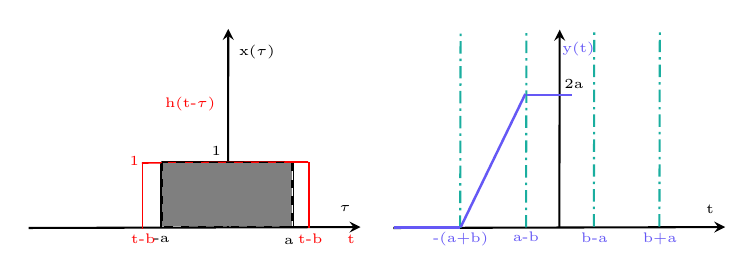
\begin{tikzpicture}[scale = 0.8]
		\pgftransformxscale{1.000000}
		\pgftransformyscale{-1.000000}
		\definecolor{dialinecolor}{rgb}{0.000000, 0.000000, 0.000000}
		\pgfsetstrokecolor{dialinecolor}
		\pgfsetstrokeopacity{1.000000}
		\definecolor{diafillcolor}{rgb}{1.000000, 1.000000, 1.000000}
		\pgfsetfillcolor{diafillcolor}
		\pgfsetfillopacity{1.000000}
		\pgfsetlinewidth{0.050000\du}
		\pgfsetdash{}{0pt}
		\pgfsetbuttcap
		{
			\definecolor{diafillcolor}{rgb}{0.000000, 0.000000, 0.000000}
			\pgfsetfillcolor{diafillcolor}
			\pgfsetfillopacity{1.000000}
			% was here!!!
			\pgfsetarrowsend{stealth}
			\definecolor{dialinecolor}{rgb}{0.000000, 0.000000, 0.000000}
			\pgfsetstrokecolor{dialinecolor}
			\pgfsetstrokeopacity{1.000000}
			\draw (40.002600\du,15.011800\du)--(40.014100\du,9.028390\du);
		}
		\pgfsetlinewidth{0.050000\du}
		\pgfsetdash{}{0pt}
		\pgfsetbuttcap
		{
			\definecolor{diafillcolor}{rgb}{0.000000, 0.000000, 0.000000}
			\pgfsetfillcolor{diafillcolor}
			\pgfsetfillopacity{1.000000}
			% was here!!!
			\pgfsetarrowsend{stealth}
			\definecolor{dialinecolor}{rgb}{0.000000, 0.000000, 0.000000}
			\pgfsetstrokecolor{dialinecolor}
			\pgfsetstrokeopacity{1.000000}
			\draw (34.004400\du,15.023000\du)--(43.996100\du,14.995700\du);
		}
		\pgfsetlinewidth{0.040000\du}
		\pgfsetdash{}{0pt}
		\pgfsetbuttcap
		{
			\definecolor{diafillcolor}{rgb}{0.000000, 0.000000, 0.000000}
			\pgfsetfillcolor{diafillcolor}
			\pgfsetfillopacity{1.000000}
			% was here!!!
			\definecolor{dialinecolor}{rgb}{0.000000, 0.000000, 0.000000}
			\pgfsetstrokecolor{dialinecolor}
			\pgfsetstrokeopacity{1.000000}
			\draw (37.996700\du,15.011800\du)--(37.996700\du,13.028800\du);
		}
		\pgfsetlinewidth{0.040000\du}
		\pgfsetdash{}{0pt}
		\pgfsetbuttcap
		{
			\definecolor{diafillcolor}{rgb}{0.000000, 0.000000, 0.000000}
			\pgfsetfillcolor{diafillcolor}
			\pgfsetfillopacity{1.000000}
			% was here!!!
			\definecolor{dialinecolor}{rgb}{0.000000, 0.000000, 0.000000}
			\pgfsetstrokecolor{dialinecolor}
			\pgfsetstrokeopacity{1.000000}
			\draw (41.980400\du,14.986000\du)--(41.980400\du,13.002900\du);
		}
		\pgfsetlinewidth{0.040000\du}
		\pgfsetdash{}{0pt}
		\pgfsetbuttcap
		{
			\definecolor{diafillcolor}{rgb}{0.000000, 0.000000, 0.000000}
			\pgfsetfillcolor{diafillcolor}
			\pgfsetfillopacity{1.000000}
			% was here!!!
			\definecolor{dialinecolor}{rgb}{0.000000, 0.000000, 0.000000}
			\pgfsetstrokecolor{dialinecolor}
			\pgfsetstrokeopacity{1.000000}
			\draw (37.996700\du,13.034500\du)--(42.011100\du,13.038400\du);
		}
		% setfont left to latex
		\definecolor{dialinecolor}{rgb}{0.000000, 0.000000, 0.000000}
		\pgfsetstrokecolor{dialinecolor}
		\pgfsetstrokeopacity{1.000000}
		\definecolor{diafillcolor}{rgb}{0.000000, 0.000000, 0.000000}
		\pgfsetfillcolor{diafillcolor}
		\pgfsetfillopacity{1.000000}
		\node[anchor=base,inner sep=0pt, outer sep=0pt,color=dialinecolor] at (38.000000\du,15.471175\du){\tiny -a};
		% setfont left to latex
		\definecolor{dialinecolor}{rgb}{0.000000, 0.000000, 0.000000}
		\pgfsetstrokecolor{dialinecolor}
		\pgfsetstrokeopacity{1.000000}
		\definecolor{diafillcolor}{rgb}{0.000000, 0.000000, 0.000000}
		\pgfsetfillcolor{diafillcolor}
		\pgfsetfillopacity{1.000000}
		\node[anchor=base east,inner sep=0pt, outer sep=0pt,color=dialinecolor] at (39.799200\du,12.850046\du){\tiny 1};
		% setfont left to latex
		\definecolor{dialinecolor}{rgb}{0.000000, 0.000000, 0.000000}
		\pgfsetstrokecolor{dialinecolor}
		\pgfsetstrokeopacity{1.000000}
		\definecolor{diafillcolor}{rgb}{0.000000, 0.000000, 0.000000}
		\pgfsetfillcolor{diafillcolor}
		\pgfsetfillopacity{1.000000}
		\node[anchor=base,inner sep=0pt, outer sep=0pt,color=dialinecolor] at (43.532700\du,14.528504\du){\tiny $\tau	$};
		% setfont left to latex
		\definecolor{dialinecolor}{rgb}{0.000000, 0.000000, 0.000000}
		\pgfsetstrokecolor{dialinecolor}
		\pgfsetstrokeopacity{1.000000}
		\definecolor{diafillcolor}{rgb}{0.000000, 0.000000, 0.000000}
		\pgfsetfillcolor{diafillcolor}
		\pgfsetfillopacity{1.000000}
		\node[anchor=base west,inner sep=0pt,outer sep=0pt,color=dialinecolor] at (40.337300\du,9.823361\du){\tiny x($\tau$)};
		\pgfsetlinewidth{0.040000\du}
		\pgfsetdash{}{0pt}
		\pgfsetbuttcap
		{
			\definecolor{diafillcolor}{rgb}{1.000000, 0.000000, 0.000000}
			\pgfsetfillcolor{diafillcolor}
			\pgfsetfillopacity{1.000000}
			% was here!!!
			\definecolor{dialinecolor}{rgb}{1.000000, 0.000000, 0.000000}
			\pgfsetstrokecolor{dialinecolor}
			\pgfsetstrokeopacity{1.000000}
			\draw (37.429316\du,15.042600\du)--(37.429316\du,13.059600\du);
		}
		\pgfsetlinewidth{0.040000\du}
		\pgfsetdash{}{0pt}
		\pgfsetbuttcap
		{
			\definecolor{diafillcolor}{rgb}{1.000000, 0.000000, 0.000000}
			\pgfsetfillcolor{diafillcolor}
			\pgfsetfillopacity{1.000000}
			% was here!!!
			\definecolor{dialinecolor}{rgb}{1.000000, 0.000000, 0.000000}
			\pgfsetstrokecolor{dialinecolor}
			\pgfsetstrokeopacity{1.000000}
			\draw (42.444716\du,15.016700\du)--(42.444716\du,13.033700\du);
		}
		\pgfsetlinewidth{0.040000\du}
		\pgfsetdash{}{0pt}
		\pgfsetbuttcap
		{
			\definecolor{diafillcolor}{rgb}{1.000000, 0.000000, 0.000000}
			\pgfsetfillcolor{diafillcolor}
			\pgfsetfillopacity{1.000000}
			% was here!!!
			\definecolor{dialinecolor}{rgb}{1.000000, 0.000000, 0.000000}
			\pgfsetstrokecolor{dialinecolor}
			\pgfsetstrokeopacity{1.000000}
			\draw (37.411638\du,13.065300\du)--(42.420938\du,13.034500\du);
		}
		% setfont left to latex
		\definecolor{dialinecolor}{rgb}{1.000000, 0.000000, 0.000000}
		\pgfsetstrokecolor{dialinecolor}
		\pgfsetstrokeopacity{1.000000}
		\definecolor{diafillcolor}{rgb}{1.000000, 0.000000, 0.000000}
		\pgfsetfillcolor{diafillcolor}
		\pgfsetfillopacity{1.000000}
		\node[anchor=base,inner sep=0pt, outer sep=0pt,color=dialinecolor] at (37.453271\du,15.492375\du){\tiny t-b};
		% setfont left to latex
		\definecolor{dialinecolor}{rgb}{1.000000, 0.000000, 0.000000}
		\pgfsetstrokecolor{dialinecolor}
		\pgfsetstrokeopacity{1.000000}
		\definecolor{diafillcolor}{rgb}{1.000000, 0.000000, 0.000000}
		\pgfsetfillcolor{diafillcolor}
		\pgfsetfillopacity{1.000000}
		\node[anchor=base,inner sep=0pt, outer sep=0pt,color=dialinecolor] at (42.487371\du,15.492375\du){\tiny t-b};
		% setfont left to latex
		\definecolor{dialinecolor}{rgb}{1.000000, 0.000000, 0.000000}
		\pgfsetstrokecolor{dialinecolor}
		\pgfsetstrokeopacity{1.000000}
		\definecolor{diafillcolor}{rgb}{1.000000, 0.000000, 0.000000}
		\pgfsetfillcolor{diafillcolor}
		\pgfsetfillopacity{1.000000}
		\node[anchor=base east,inner sep=0pt, outer sep=0pt,color=dialinecolor] at (37.330271\du,13.134346\du){\tiny 1};
		% setfont left to latex
		\definecolor{dialinecolor}{rgb}{1.000000, 0.000000, 0.000000}
		\pgfsetstrokecolor{dialinecolor}
		\pgfsetstrokeopacity{1.000000}
		\definecolor{diafillcolor}{rgb}{1.000000, 0.000000, 0.000000}
		\pgfsetfillcolor{diafillcolor}
		\pgfsetfillopacity{1.000000}
		\node[anchor=base west,inner sep=0pt,outer sep=0pt,color=dialinecolor] at (38.110178\du,11.406131\du){\tiny h(t-$\tau$)};
		% setfont left to latex
		\definecolor{dialinecolor}{rgb}{1.000000, 0.000000, 0.000000}
		\pgfsetstrokecolor{dialinecolor}
		\pgfsetstrokeopacity{1.000000}
		\definecolor{diafillcolor}{rgb}{1.000000, 0.000000, 0.000000}
		\pgfsetfillcolor{diafillcolor}
		\pgfsetfillopacity{1.000000}
		\node[anchor=base,inner sep=0pt, outer sep=0pt,color=dialinecolor] at (43.715100\du,15.482117\du){\tiny t};
		\pgfsetlinewidth{0.030000\du}
		\pgfsetdash{{0.200000\du}{0.200000\du}}{0\du}
		\pgfsetmiterjoin
		\pgfsetbuttcap
		{\pgfsetcornersarced{\pgfpoint{0.000000\du}{0.000000\du}}\definecolor{diafillcolor}{rgb}{0.498039, 0.498039, 0.498039}
			\pgfsetfillcolor{diafillcolor}
			\pgfsetfillopacity{1.000000}
			\fill (38.015698\du,13.053200\du)--(38.015698\du,14.977486\du)--(41.932323\du,14.977486\du)--(41.932323\du,13.053200\du)--cycle;
		}{\pgfsetcornersarced{\pgfpoint{0.000000\du}{0.000000\du}}\definecolor{dialinecolor}{rgb}{0.000000, 0.000000, 0.000000}
			\pgfsetstrokecolor{dialinecolor}
			\pgfsetstrokeopacity{1.000000}
			\draw (38.015698\du,13.053200\du)--(38.015698\du,14.977486\du)--(41.932323\du,14.977486\du)--(41.932323\du,13.053200\du)--cycle;
		}\pgfsetlinewidth{0.050000\du}
		\pgfsetdash{}{0pt}
		\pgfsetbuttcap
		{
			\definecolor{diafillcolor}{rgb}{0.000000, 0.000000, 0.000000}
			\pgfsetfillcolor{diafillcolor}
			\pgfsetfillopacity{1.000000}
			% was here!!!
			\pgfsetarrowsend{stealth}
			\definecolor{dialinecolor}{rgb}{0.000000, 0.000000, 0.000000}
			\pgfsetstrokecolor{dialinecolor}
			\pgfsetstrokeopacity{1.000000}
			\draw (44.986300\du,15.023300\du)--(54.978000\du,14.996000\du);
		}
		\pgfsetlinewidth{0.050000\du}
		\pgfsetdash{}{0pt}
		\pgfsetbuttcap
		{
			\definecolor{diafillcolor}{rgb}{0.000000, 0.000000, 0.000000}
			\pgfsetfillcolor{diafillcolor}
			\pgfsetfillopacity{1.000000}
			% was here!!!
			\pgfsetarrowsend{stealth}
			\definecolor{dialinecolor}{rgb}{0.000000, 0.000000, 0.000000}
			\pgfsetstrokecolor{dialinecolor}
			\pgfsetstrokeopacity{1.000000}
			\draw (49.982100\du,15.009600\du)--(49.993900\du,9.052460\du);
		}
		\pgfsetlinewidth{0.050000\du}
		\pgfsetdash{{0.300000\du}{0.120000\du}{0.060000\du}{0.120000\du}}{0cm}
		\pgfsetbuttcap
		{
			\definecolor{diafillcolor}{rgb}{0.101961, 0.682353, 0.623529}
			\pgfsetfillcolor{diafillcolor}
			\pgfsetfillopacity{1.000000}
			% was here!!!
			\definecolor{dialinecolor}{rgb}{0.101961, 0.682353, 0.623529}
			\pgfsetstrokecolor{dialinecolor}
			\pgfsetstrokeopacity{1.000000}
			\draw (46.996400\du,15.021100\du)--(47.008100\du,9.063880\du);
		}
		\pgfsetlinewidth{0.050000\du}
		\pgfsetdash{{0.300000\du}{0.120000\du}{0.060000\du}{0.120000\du}}{0cm}
		\pgfsetbuttcap
		{
			\definecolor{diafillcolor}{rgb}{0.101961, 0.682353, 0.623529}
			\pgfsetfillcolor{diafillcolor}
			\pgfsetfillopacity{1.000000}
			% was here!!!
			\definecolor{dialinecolor}{rgb}{0.101961, 0.682353, 0.623529}
			\pgfsetstrokecolor{dialinecolor}
			\pgfsetstrokeopacity{1.000000}
			\draw (48.980200\du,15.007400\du)--(48.992000\du,9.050250\du);
		}
		\pgfsetlinewidth{0.050000\du}
		\pgfsetdash{{0.300000\du}{0.120000\du}{0.060000\du}{0.120000\du}}{0cm}
		\pgfsetbuttcap
		{
			\definecolor{diafillcolor}{rgb}{0.101961, 0.682353, 0.623529}
			\pgfsetfillcolor{diafillcolor}
			\pgfsetfillopacity{1.000000}
			% was here!!!
			\definecolor{dialinecolor}{rgb}{0.101961, 0.682353, 0.623529}
			\pgfsetstrokecolor{dialinecolor}
			\pgfsetstrokeopacity{1.000000}
			\draw (51.022200\du,14.980200\du)--(51.033900\du,9.022980\du);
		}
		\pgfsetlinewidth{0.050000\du}
		\pgfsetdash{{0.300000\du}{0.120000\du}{0.060000\du}{0.120000\du}}{0cm}
		\pgfsetbuttcap
		{
			\definecolor{diafillcolor}{rgb}{0.101961, 0.682353, 0.623529}
			\pgfsetfillcolor{diafillcolor}
			\pgfsetfillopacity{1.000000}
			% was here!!!
			\definecolor{dialinecolor}{rgb}{0.101961, 0.682353, 0.623529}
			\pgfsetstrokecolor{dialinecolor}
			\pgfsetstrokeopacity{1.000000}
			\draw (52.996000\du,14.980200\du)--(53.007700\du,9.022980\du);
		}
		\pgfsetlinewidth{0.060000\du}
		\pgfsetdash{}{0pt}
		\pgfsetbuttcap
		{
			\definecolor{diafillcolor}{rgb}{0.396078, 0.345098, 0.960784}
			\pgfsetfillcolor{diafillcolor}
			\pgfsetfillopacity{1.000000}
			% was here!!!
			\definecolor{dialinecolor}{rgb}{0.396078, 0.345098, 0.960784}
			\pgfsetstrokecolor{dialinecolor}
			\pgfsetstrokeopacity{1.000000}
			\draw (45.005200\du,15.011200\du)--(46.988200\du,15.011200\du);
		}
		\pgfsetlinewidth{0.060000\du}
		\pgfsetdash{}{0pt}
		\pgfsetbuttcap
		{
			\definecolor{diafillcolor}{rgb}{0.396078, 0.345098, 0.960784}
			\pgfsetfillcolor{diafillcolor}
			\pgfsetfillopacity{1.000000}
			% was here!!!
			\definecolor{dialinecolor}{rgb}{0.396078, 0.345098, 0.960784}
			\pgfsetstrokecolor{dialinecolor}
			\pgfsetstrokeopacity{1.000000}
			\draw (47.011200\du,14.999700\du)--(48.958144\du,10.988487\du);
		}
		% setfont left to latex
		\definecolor{dialinecolor}{rgb}{0.396078, 0.345098, 0.960784}
		\pgfsetstrokecolor{dialinecolor}
		\pgfsetstrokeopacity{1.000000}
		\definecolor{diafillcolor}{rgb}{0.396078, 0.345098, 0.960784}
		\pgfsetfillcolor{diafillcolor}
		\pgfsetfillopacity{1.000000}
		\node[anchor=base,inner sep=0pt, outer sep=0pt,color=dialinecolor] at (47.009500\du,15.451675\du){\tiny -(a+b)};
		% setfont left to latex
		\definecolor{dialinecolor}{rgb}{0.396078, 0.345098, 0.960784}
		\pgfsetstrokecolor{dialinecolor}
		\pgfsetstrokeopacity{1.000000}
		\definecolor{diafillcolor}{rgb}{0.396078, 0.345098, 0.960784}
		\pgfsetfillcolor{diafillcolor}
		\pgfsetfillopacity{1.000000}
		\node[anchor=base,inner sep=0pt, outer sep=0pt,color=dialinecolor] at (48.976600\du,15.440175\du){\tiny a-b};
		% setfont left to latex
		\definecolor{dialinecolor}{rgb}{0.396078, 0.345098, 0.960784}
		\pgfsetstrokecolor{dialinecolor}
		\pgfsetstrokeopacity{1.000000}
		\definecolor{diafillcolor}{rgb}{0.396078, 0.345098, 0.960784}
		\pgfsetfillcolor{diafillcolor}
		\pgfsetfillopacity{1.000000}
		\node[anchor=base,inner sep=0pt, outer sep=0pt,color=dialinecolor] at (51.037500\du,15.451675\du){\tiny b-a};
		% setfont left to latex
		\definecolor{dialinecolor}{rgb}{0.396078, 0.345098, 0.960784}
		\pgfsetstrokecolor{dialinecolor}
		\pgfsetstrokeopacity{1.000000}
		\definecolor{diafillcolor}{rgb}{0.396078, 0.345098, 0.960784}
		\pgfsetfillcolor{diafillcolor}
		\pgfsetfillopacity{1.000000}
		\node[anchor=base,inner sep=0pt, outer sep=0pt,color=dialinecolor] at (53.006800\du,15.451675\du){\tiny b+a};
		% setfont left to latex
		\definecolor{dialinecolor}{rgb}{0.000000, 0.000000, 0.000000}
		\pgfsetstrokecolor{dialinecolor}
		\pgfsetstrokeopacity{1.000000}
		\definecolor{diafillcolor}{rgb}{0.000000, 0.000000, 0.000000}
		\pgfsetfillcolor{diafillcolor}
		\pgfsetfillopacity{1.000000}
		\node[anchor=base,inner sep=0pt, outer sep=0pt,color=dialinecolor] at (54.525900\du,14.580517\du){\tiny t};
		% setfont left to latex
		\definecolor{dialinecolor}{rgb}{0.000000, 0.000000, 0.000000}
		\pgfsetstrokecolor{dialinecolor}
		\pgfsetstrokeopacity{1.000000}
		\definecolor{diafillcolor}{rgb}{0.000000, 0.000000, 0.000000}
		\pgfsetfillcolor{diafillcolor}
		\pgfsetfillopacity{1.000000}
		\node[anchor=base,inner sep=0pt, outer sep=0pt,color=dialinecolor] at (50.420800\du,10.820775\du){\tiny 2a};
		% setfont left to latex
		\definecolor{dialinecolor}{rgb}{0.396078, 0.345098, 0.960784}
		\pgfsetstrokecolor{dialinecolor}
		\pgfsetstrokeopacity{1.000000}
		\definecolor{diafillcolor}{rgb}{0.396078, 0.345098, 0.960784}
		\pgfsetfillcolor{diafillcolor}
		\pgfsetfillopacity{1.000000}
		\node[anchor=base,inner sep=0pt, outer sep=0pt,color=dialinecolor] at (50.558400\du,9.743345\du){\tiny y(t)};
		% setfont left to latex
		\definecolor{dialinecolor}{rgb}{0.000000, 0.000000, 0.000000}
		\pgfsetstrokecolor{dialinecolor}
		\pgfsetstrokeopacity{1.000000}
		\definecolor{diafillcolor}{rgb}{0.000000, 0.000000, 0.000000}
		\pgfsetfillcolor{diafillcolor}
		\pgfsetfillopacity{1.000000}
		\node[anchor=base,inner sep=0pt, outer sep=0pt,color=dialinecolor] at (41.836293\du,15.519991\du){\tiny a};
		\pgfsetlinewidth{0.060000\du}
		\pgfsetdash{}{0pt}
		\pgfsetbuttcap
		{
			\definecolor{diafillcolor}{rgb}{0.396078, 0.345098, 0.960784}
			\pgfsetfillcolor{diafillcolor}
			\pgfsetfillopacity{1.000000}
			% was here!!!
			\definecolor{dialinecolor}{rgb}{0.396078, 0.345098, 0.960784}
			\pgfsetstrokecolor{dialinecolor}
			\pgfsetstrokeopacity{1.000000}
			\draw (48.993499\du,11.015003\du)--(50.372353\du,11.015003\du);
		}
	\end{tikzpicture}
	\vspace{-2mm}
	\caption{\scriptsize Traslape segmento constante.}
	\label{fig:traslape2}
\end{figure}
